% ----------------------------------
% File    : cruz_computing_2020_04_template.tex
% Content : Template section of the article for Computing
% Date    : 1/12/2018
% Authors : M.Cruz
% ----------------------------------

% ----------------------------------
% Last update: 10/11/2020 (MCruz)
% Actualización a partir de la tesis
% ----------------------------------

%----------------------------------
\section{Template for specifying changes in replications}
\label{sec:plantilla}
%----------------------------------

This section develops a possible visual representation of the meta--model through a template. 
The template has a double purpose: on the one hand, it motivates the researcher to make the change and its details explicit (reducing \emph{tacit knowledge}) and, on the other hand, it helps the reader to better understand the replication and to follow the trace of how the original experiment evolves in the succession of experiments across a family of them.

The template is completed with L-patterns. They are common phrases identified and parameterized for some fields in the template \cite{duran2002supporting}.
In the notation used to describe the L-patterns, words or phrases between \textless \hspace{0.5 mm} and \textgreater \hspace{1 mm} must be properly replaced.
Words or phrases between \{ and \} and separated by \textbar \hspace{1 mm} represents options, only one option must be chosen.
Words between [ and ]$^+$ are repeated 1 or more times; that is, they appear at least once but there may be more than one occurrence
and between [ and ] are optional.

Filling the blanks in pre–written sentences, i.e. L–patterns, is easier and faster than writing a whole paragraph. 

%-----------------------
\begin{figure*}[h]
    %\centering
    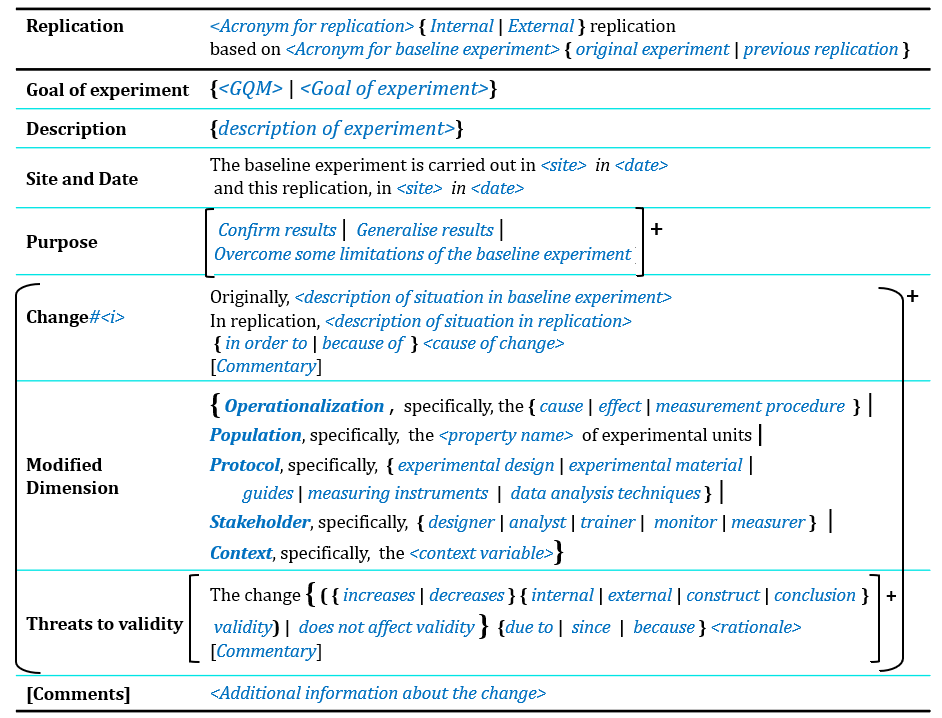
\includegraphics[width=1\textwidth]{figures/Template.png}
    \caption{Template to specfy changes in a replication}
    \label{fig:Template-V1} 
\end{figure*}
%-----------------------



Fig.~\ref{fig:Template-V1} shows the proposed template.
The template consists of two clearly differentiated parts: a general part for the specification of \textit{basic aspects} of replication and a specific part for each of the \textit{changes} included in the replication.

